\documentclass[11pt,fleqn]{article} 
\usepackage[margin=0.8in, head=0.8in]{geometry} 
\usepackage{amsmath, amssymb, amsthm}
\usepackage{fancyhdr} 
\usepackage{palatino, url, multicol}
\usepackage{graphicx, pgfplots} 
\usepackage[all]{xy}
\usepackage{polynom} 
%\usepackage{pdfsync} %% I don't know why this messes up tabular column widths
\usepackage{enumerate}
\usepackage{framed}
\usepackage{setspace}
\usepackage{array}
\usepackage{pgf,tikz}
\usepackage{mathrsfs}
\usetikzlibrary{arrows}

\usetikzlibrary{calc}

\pgfplotsset{compat=1.6}

\pgfplotsset{soldot/.style={color=blue,only marks,mark=*}} \pgfplotsset{holdot/.style={color=blue,fill=white,only marks,mark=*}}

\renewcommand{\headrulewidth}{0pt}
\newcommand{\blank}[1]{\rule{#1}{0.75pt}}
\newcommand{\bc}{\begin{center}}
\newcommand{\ec}{\end{center}}
\newcommand{\be}{\begin{enumerate}}
\newcommand{\ee}{\end{enumerate}}

\newcommand{\ds}{\displaystyle}



\pagestyle{fancy} 
%\lfoot{Uses a calculator}
\rfoot{4-3 }

\begin{document}
\begin{center}
  \large
  \sc{Section 4-3: How Derivatives Affect the Shape of a Graph}\\
\end{center}

\textbf{Mean Value Theorem.}\hskip 1ex If $f$ is a continuous function on an interval
$[a,b]$ that has a derivative at every point in $(a,b)$, then there
is a point $c$ in $(a,b)$ where
$$
f'(c) = \frac{f(b)-f(a)}{b-a}.
$$

\be

\item Suppose $f$ is a continuous function on $[a,b]$ that
has a derivative at every point of $(a,b)$.  Suppose also that
$f(b) \le f(a)$.  What can you conclude from the Mean Value Theorem?
\vfill
\item Suppose $f$ is a continuous function on $[a,b]$ that
has a derivative at every point of $(a,b)$, and that $f'(x)>0$
for each $x$ in $(a,b)$.  Thinking about your answer to problem 1,
what can you conclude about $f(a)$ and $f(b)$?
\vfill
\item A function is said to be \textbf{increasing} on an interval $(a,b)$
if whenever $x$ and $z$ are in the interval and $x<z$, then $f(x)<f(z)$.
It is \textbf{decreasing} if whenever 
$x$ and $z$ are in the interval and $x<z$, then $f(x)>f(z)$
Sketch an example of a function that is increasing on $(1, 3)$ and
decreasing on $(3,5)$.
\vfill
\newpage
\textbf{Increasing/Decreasing Test}\\ 
Your answer to problem 2 implies the first item below; the second is
justified by a similar argument.
\begin{itemize}
\item If $f'(x)>0$ on an interval $(a,b)$ then $f$ is increasing on the interval.
\item If $f'(x)<0$ on an interval $(a,b)$ then $f$ is decreasing on the interval.
\end{itemize}
\item
Use the increasing/decreasing test to find intervals where
\[
f(x) = \frac{2}{3}x^3 +x^2 -12 x + 7
\]
is increasing and intervals where it is decreasing.
\vfill

\item Find the critical points of the function
$\ds f(x)=\frac{2}{3}x^3 +x^2 -12 x + 7$ from the previous problem.
There should be two, $c_1$ and $c_2$ with $c_1<c_2$.  
Just pay attention to $c_1$.  
\begin{enumerate}
	\item Just to the left of $c_1$ is the function increasing or decreasing?
	\item Just to the right of $c_1$ is the function increasing or decreasing?
	\item Now decide intuitively, based on these two observations, if $f$ has a local min, local max, or neither at $c_1$.
\end{enumerate}
\vfill
\item Repeat the previous exercise for the other critical point $c_2$.
\vfill
\newpage
You have just sketched the argument that justifies the following:

\textbf{First Derivative Test}\\
Suppose $f$ is a function with a derivative on $(a,b)$, and if $c$ is a
point in the interval with $f'(c)=0$.
\begin{itemize}
\item If
$f'(x)>0$ for $x$ just to the left of $c$ and
$f'(x)<0$ for $x$ just to the right of $c$, then $f$ has a \rule{0pt}{1.5\baselineskip}\blank{1.5in} at $c$.
\vskip 1cm
\item If
$f'(x)<0$ for $x$ just to the left of $c$ and
$f'(x)>0$ for $x$ just to the right of $c$, then $f$ has a 
\rule{0pt}{1.5\baselineskip}\blank{1.5in} at $c$.
\vskip 1cm
\end{itemize}
\item The function $f(x)=xe^x$ has exactly one critical point.
Find it, and then use the First Derivative Test to determine if a local
minimum or local maximum occurs there.
\vfill
\item Consider the function $f(x)=\frac{2}{3}x^3 +x^2 -12 x + 7$.
Find intervals such that the \textbf{derivative} of $f(x)$ is increasing or decreasing.
\vfill
\item Earlier you computed that $f'(-3)=0$.  Is $f'$ increasing near $x=-3$
or decreasing near $x=-3$?  Which of the following two scenarios must we have?\vskip 1cm
\hfill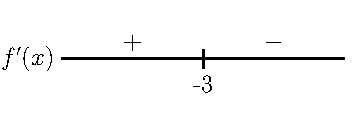
\includegraphics{Fig-4-3a.pdf}\hfill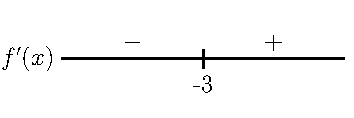
\includegraphics{Fig-4-3b.pdf}\hfill
\newpage
You have just sketched out justification for the following.

\textbf{Second Derivative Test}\\
Suppose $f$ is a function with a continuous second derivative on $(a,b)$, and that $c$ is a point in the interval with $f'(c)=0$.
\begin{itemize}
\item If $f''(c)>0$ then $f$ has a \blank{1.5in} at $c$.
\vskip 1cm
\item If $f''(c)<0$ then $f$ has a \blank{1.5in} at $c$.
\vskip 1cm
\end{itemize}

\item Use the Second Derivative Test to determine if $f(x)=xe^x$ has
a local min/max at its only critical point.
\vfill
\item Consider the function $f(x)=x^3$.  Verify that $f'(0)=0$.
Then decide what the Second Derivative Test has to say, if anything,
about whether a local min/max occurs at $x=0$.
\vfill
\item Decide what the First Derivative Test has to say, if anything,
about whether a local min/max occurs at $x=0$ for $f(x)=x^3$.
\vfill
\ee
\end{document}
